\section{Resultater}

\subsection{Informasjon om informantene}
\subsubsection{Hvilket kjønn er du?}
\begin{figure}[H]
    \centering
    \begin{tikzpicture}
        \pie[color = {blue!65!green,red!60,yellow!60,orange!70,green!60!black,teal!50}]{
            54  /San Antonio Spurs,
            46  /Other Teams}
    \end{tikzpicture}    
    \caption{Test}
\end{figure}

\subsubsection{Hvor gammel er du?}
\begin{figure}[H]
    \centering
    \begin{tikzpicture}
        \pie[color = {blue!65!green,red!60,yellow!60,orange!70,green!60!black,teal!50},
        explode = {0.4, 0, 0.4, 0, 0},
        pos = {0,0}]{
            24    /Los Angeles Lakers,
            30  /Boston Celtics,
            17    /Chicago Bulls,
            11  /San Antonio Spurs,
            18    /Other Teams}
    \end{tikzpicture}    
    \caption{Test}
\end{figure}

\subsubsection{A}
\begin{figure}[H]
    \centering
    \begin{tikzpicture}
        \pie[color = {blue!65!green,red!60,yellow!60,orange!70,green!60!black,teal!50},
        explode = {0.4, 0, 0},
        text = inside]{
            71  /B Celtics,
            11  /SA Spurs,
            18    /Other}
        \pie[color = {blue!65!green,red!60,yellow!60,orange!70,green!60!black,teal!50},
        explode = {0},
        pos = {7,0},
        text = inside]{
            24    /LA Lakers,
            30  /B Celtics,
            17    /C Bulls,
            11  /SA Spurs,
            18    /Other}
    \end{tikzpicture}    
    \caption{Test}
\end{figure}

\subsubsection{A}
\begin{figure}[H]
    \centering
    \begin{tikzpicture}
        \pie[color = {blue!65!green,red!60,yellow!60,orange!70,green!60!black,teal!50},
        explode = {0.4, 0, 0.4, 0, 0}]{
            24    /Los Angeles Lakers,
            30  /Boston Celtics,
            17    /Chicago Bulls,
            11  /San Antonio Spurs,
            18    /Other Teams}
    \end{tikzpicture}    
    \caption{Test}
\end{figure}

\subsubsection{A}
\begin{figure}[H]
    \centering
    \begin{tikzpicture}
        \pie[color = {blue!65!green,red!60,yellow!60,orange!70,green!60!black,teal!50},
        explode = {0.4, 0, 0.4, 0, 0}]{
            24    /Los Angeles Lakers,
            30  /Boston Celtics,
            17    /Chicago Bulls,
            11  /San Antonio Spurs,
            18    /Other Teams}
    \end{tikzpicture}    
    \caption{Test}
\end{figure}
    
\subsection{Generelt om personvern}
\subsubsection{A}
\begin{figure}[H]
    \centering
    \begin{tikzpicture}
        \pie[color = {blue!65!green,red!60,yellow!60,orange!70,green!60!black,teal!50},
        explode = {0.4, 0, 0.4, 0, 0}]{
            24    /Los Angeles Lakers,
            30  /Boston Celtics,
            17    /Chicago Bulls,
            11  /San Antonio Spurs,
            18    /Other Teams}
    \end{tikzpicture}    
    \caption{Test}
\end{figure}

\subsubsection{A}
\begin{figure}[H]
    \centering
    \begin{tikzpicture}
        \pie[color = {blue!65!green,red!60,yellow!60,orange!70,green!60!black,teal!50},
        explode = {0.4, 0, 0.4, 0, 0}]{
            24    /Los Angeles Lakers,
            30  /Boston Celtics,
            17    /Chicago Bulls,
            11  /San Antonio Spurs,
            18    /Other Teams}
    \end{tikzpicture}    
    \caption{Test}
\end{figure}

\subsubsection{A}
\begin{figure}[H]
    \centering
    \begin{tikzpicture}
        \pie[color = {blue!65!green,red!60,yellow!60,orange!70,green!60!black,teal!50},
        explode = {0.4, 0, 0.4, 0, 0}]{
            24    /Los Angeles Lakers,
            30  /Boston Celtics,
            17    /Chicago Bulls,
            11  /San Antonio Spurs,
            18    /Other Teams}
    \end{tikzpicture}    
    \caption{Test}
\end{figure}

\subsubsection{A}
\begin{figure}[H]
    \centering
    \begin{tikzpicture}
        \pie[color = {blue!65!green,red!60,yellow!60,orange!70,green!60!black,teal!50},
        explode = {0.4, 0, 0.4, 0, 0}]{
            24    /Los Angeles Lakers,
            30  /Boston Celtics,
            17    /Chicago Bulls,
            11  /San Antonio Spurs,
            18    /Other Teams}
    \end{tikzpicture}    
    \caption{Test}
\end{figure}

\subsubsection{A}
\begin{figure}[H]
    \centering
    \begin{tikzpicture}
        \pie[color = {blue!65!green,red!60,yellow!60,orange!70,green!60!black,teal!50},
        explode = {0.4, 0, 0.4, 0, 0}]{
            24    /Los Angeles Lakers,
            30  /Boston Celtics,
            17    /Chicago Bulls,
            11  /San Antonio Spurs,
            18    /Other Teams}
    \end{tikzpicture}    
    \caption{Test}
\end{figure}

\subsubsection{A}
\begin{figure}[H]
    \centering
    \begin{tikzpicture}
        \pie[color = {blue!65!green,red!60,yellow!60,orange!70,green!60!black,teal!50},
        explode = {0.4, 0, 0.4, 0, 0}]{
            24    /Los Angeles Lakers,
            30  /Boston Celtics,
            17    /Chicago Bulls,
            11  /San Antonio Spurs,
            18    /Other Teams}
    \end{tikzpicture}    
    \caption{Test}
\end{figure}

\subsection{Overvåkning}
\subsubsection{A}
\begin{figure}[H]
    \centering
    \begin{tikzpicture}
        \pie[color = {blue!65!green,red!60,yellow!60,orange!70,green!60!black,teal!50},
        explode = {0.4, 0, 0.4, 0, 0}]{
            24    /Los Angeles Lakers,
            30  /Boston Celtics,
            17    /Chicago Bulls,
            11  /San Antonio Spurs,
            18    /Other Teams}
    \end{tikzpicture}    
    \caption{Test}
\end{figure}

\subsubsection{A}
\begin{figure}[H]
    \centering
    \begin{tikzpicture}
        \pie[color = {blue!65!green,red!60,yellow!60,orange!70,green!60!black,teal!50},
        explode = {0.4, 0, 0.4, 0, 0}]{
            24    /Los Angeles Lakers,
            30  /Boston Celtics,
            17    /Chicago Bulls,
            11  /San Antonio Spurs,
            18    /Other Teams}
    \end{tikzpicture}    
    \caption{Test}
\end{figure}

\subsubsection{A}
\begin{figure}[H]
    \centering
    \begin{tikzpicture}
        \pie[color = {blue!65!green,red!60,yellow!60,orange!70,green!60!black,teal!50},
        explode = {0.4, 0, 0.4, 0, 0}]{
            24    /Los Angeles Lakers,
            30  /Boston Celtics,
            17    /Chicago Bulls,
            11  /San Antonio Spurs,
            18    /Other Teams}
    \end{tikzpicture}    
    \caption{Test}
\end{figure}

\subsubsection{A}
\begin{figure}[H]
    \centering
    \begin{tikzpicture}
        \pie[color = {blue!65!green,red!60,yellow!60,orange!70,green!60!black,teal!50},
        explode = {0.4, 0, 0.4, 0, 0}]{
            24    /Los Angeles Lakers,
            30  /Boston Celtics,
            17    /Chicago Bulls,
            11  /San Antonio Spurs,
            18    /Other Teams}
    \end{tikzpicture}    
    \caption{Test}
\end{figure}

\subsubsection{A}
\begin{figure}[H]
    \centering
    \begin{tikzpicture}
        \pie[color = {blue!65!green,red!60,yellow!60,orange!70,green!60!black,teal!50},
        explode = {0.4, 0, 0.4, 0, 0}]{
            24    /Los Angeles Lakers,
            30  /Boston Celtics,
            17    /Chicago Bulls,
            11  /San Antonio Spurs,
            18    /Other Teams}
    \end{tikzpicture}    
    \caption{Test}
\end{figure}

\subsubsection{A}
\begin{figure}[H]
    \centering
    \begin{tikzpicture}
        \pie[color = {blue!65!green,red!60,yellow!60,orange!70,green!60!black,teal!50},
        explode = {0.4, 0, 0.4, 0, 0}]{
            24    /Los Angeles Lakers,
            30  /Boston Celtics,
            17    /Chicago Bulls,
            11  /San Antonio Spurs,
            18    /Other Teams}
    \end{tikzpicture}    
    \caption{Test}
\end{figure}


\begin{figure}[H]
    \centering
    \begin{center}
        \emph{Hvilken kjønn er du?}
    \end{center}
    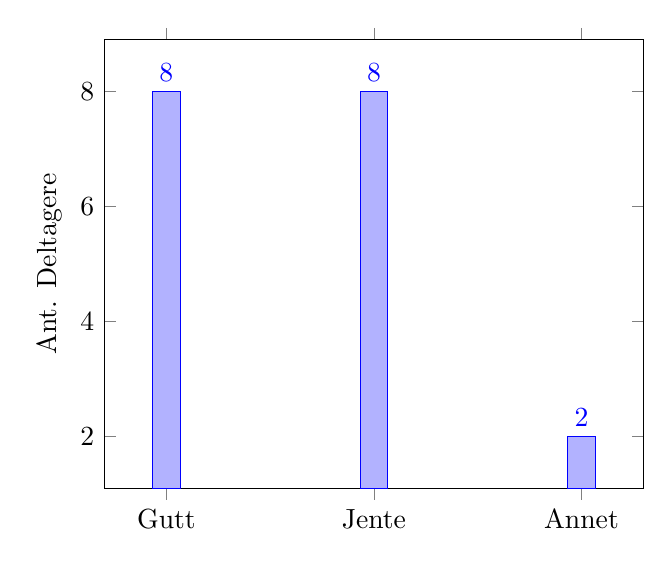
\begin{tikzpicture}
        \begin{axis}[ybar, enlargelimits=0.15, legend style={at={(0.5,-0.2)},
            anchor=north, legend columns=-1}, ylabel={Ant. Deltagere},
            symbolic x coords={Gutt, Jente, Annet}, xtick=data,
            nodes near coords, nodes near coords align={vertical},]
            % x tick label style={rotate=15, anchor=east},]
            \addplot coordinates {(Gutt, 8) (Jente, 8) (Annet, 2)};
        \end{axis}
    \end{tikzpicture}
    \caption{Test}
\end{figure}

\newpage